%XeTeX
\documentclass[a4paper, 11pt, titlepage]{article}
\usepackage{microtype}
\usepackage{a4wide}
\usepackage{import}

%Font stuff
%\usepackage{fontspec}
%\setmainfont[Ligatures={TeX}]{Source Serif Pro}

%Harvard referencing
\usepackage[authoryear]{natbib}

%Margins
\usepackage[top=2.5cm, bottom=2.5cm, left=2.5cm, right=2.5cm]{geometry}
%\renewcommand{\baselinestretch}{1.2}

%No paragraph indenting
\usepackage{parskip}
\usepackage{titlesec}
\titlespacing\section{0pt}{4pt}{5pt}
\titlespacing\subsection{0pt}{4pt}{2pt}
\titlespacing\subsubsection{0pt}{2pt}{2pt}
\parskip 8.2pt 
%So we can have a paragraph depth to 4
\setcounter{secnumdepth}{4}
\titleformat{\paragraph}
{\normalfont\normalsize\bfseries}{\theparagraph}{1em}{}
\titlespacing*{\paragraph}
{0pt}{3.25ex plus 1ex minus .2ex}{1.5ex plus .2ex}

%Whole paragraph indent
\usepackage{changepage}

%List spacing
%\usepackage{enumitem}

%Headers
\usepackage{fancyhdr}
\pagestyle{fancy}
\fancyhead{}
\fancyfoot{}

\fancyhead[LO, L]{}
\fancyfoot[CO, C]{\thepage}

%PDF hyperlinks
\usepackage{xcolor}
\definecolor{brown}{HTML}{85661E}
\definecolor{maroon}{HTML}{800B0B}
\definecolor{navyblue}{HTML}{1E5A9C}
\usepackage{hyperref}
\hypersetup{
     colorlinks		= true,
     citecolor		= black,
     linkcolor		= maroon,
     urlcolor		= navyblue,
     bookmarksopen	= false,
     pdfpagemode	= UseNone,
     pdftitle		= {CITS3200N Requirements Analysis Document},
     pdfauthor		= {CITS3200 Group N 2014},
     pdfsubject	= {Deliverable A}
}

%Figures
\usepackage{float}
\usepackage{graphicx}

%Lorem ipsum
\usepackage{lipsum}

%MS Word 1.5 line spacing
\linespread{1.3}

%Table that spans the width of the page
\usepackage{tabularx}
%\newenvironment{spanning}[1]
%	{\begin{tabular*}{\textwidth}{@{\extracolsep{\fill}} #1}}
%	{\end{tabular*}}


\begin{document}
\begin{center}
CITS3200 - Professional Computing\par
{\bf \Large Requirements Analysis Document} \par
CITS3200 Group N --- Training, Nutrition and Psychology Data Collection\\
August 2014
\end{center}

\subsection*{Revision History}
\begin{table}[H]
\begin{tabularx}{\textwidth}{|lllX|}
\hline
Version & Author & Date & Description \\
\hline
0.1 & Stuart Paton & 13 August 2014 & Initial version \\
0.2 &  & 22 August 2014 & Deliverable A \\
0.3 & & 5 September 2014 & Deliverable B \\
\hline
\end{tabularx}
\end{table}

\subsection*{Preface}
This document addresses the requirements of the iPhone/iPad Training, Nutrition and Psychology Data Collection Project. The intended audience for this document are the designers and the clients of the project.

\subsection*{Target Audience}
Client, Developers

\subsection*{Client sign-off}
I, Grant Landers have reviewed and approve of the Requirements Analysis Document, where the information outlined is accurate and suited to my needs. I accept this document as the basis for undertaking this project.  \\[2em]
\noindent \begin{tabular}{ll}
\makebox[6cm]{\hrulefill} & \makebox[6cm]{\hrulefill} \\
Signature & Date
\end{tabular}

If there are any outstanding issues, or if you would like to make changes, additions or deletions to this document, please annotate these as necessary.


\subsection*{CITS3200 Group N Members}
\begin{table}[H]
\centering
\begin{tabular}{lcl}
	\hline
	Name & Student Number & Role \\
	\hline
	Stuart Paton & 20148763  & Group manager\\
	Hillary Loh & 20517519 & Developer\\
	Kian Aik (Johnathan) Lim & 20687818 & Developer \\
	Joel Frewin & 21306458 & Developer\\
	Jeremy Tan & 20933708 & Developer\\
\end{tabular}
\end{table}

\pagenumbering{roman}

\pagebreak

%-------------------------------------------------------------------------------

\subsection*{Meeting schedule}
\begin{table}[H]
\begin{tabularx}{\textwidth}{lll}
\hline
Date & Time & Description \\
\hline
31/07/2014 & 11AM--12PM & Group Meeting \\
04/08/2014 & 12PM--1PM & Group Meeting \\
05/08/2014 & 12PM--1PM & Group Meeting and subsequent Client Meeting \\
11/08/2014 & 12:30PM--1PM & Group Meeting \\
18/08/2014 & 3PM--4:30PM & Group Meeting \\
25/08/2014 & 3PM--4PM & Group Meeting \\
26/08/2014 & 11AM-12PM & Group Meeting \\
26/08/2014 & 1PM--1:30PM & Client Meeting \\
02/09/2014 & 11AM--12PM & Group Meeting \\
02/09/2014 & 1PM--?? & Client Meeting
\end{tabularx}
\end{table}

Weekly group meetings are to be held every Monday from the August 4 2014 until October 27 2014. 

Client meetings will be scheduled on an as-needed basis with the client.

\pagebreak

%-------------------------------------------------------------------------------
% Do the table of Contents and lists of figures and tables
%-------------------------------------------------------------------------------
\begingroup
\linespread{0.7}
\hypersetup{linkcolor=black}
\tableofcontents
\endgroup

\pagebreak
\pagenumbering{arabic}
%-------------------------------------------------------------------------------

\section{General Goals}
The goal is to develop a mobile application that makes it easier to collect data from users, for the purpose of fitness and training studies at UWA.

The system is designed to streamline data entry from the client, such that the collected data is as up to date and accurate as possible. It should reduce the manual transfer of data as much as possible, both to minimise transcription errors and to increase data processing efficiency. 

\section{Current System}
The current system involves filling out paper forms, which have to be printed and gathered. This is a significant time investment and often includes half-remembered data. 

Those forms are then manually copied to an Excel spreadsheet, where various statistical analyses are performed. This manual process leads to a slow turnaround from when the data is recorded to when it is analysed.

\section{Proposed System}
\subsection{Overview}
A mobile application (app) will replace the paper forms, encouraging users to enter data sooner rather than later. The second component is a server backend, which the application will connect to remotely; most likely over the internet. Its function is to manage the users of the application, as well as to retrieve and store the data from users. The third component is an administrative interface to manage the system.

\subsection{Functional Requirements}
% Table generated by Excel2LaTeX from sheet 'Sheet1'
\begin{table}[H]
  \centering
    \begin{tabularx}{\textwidth}{lrXrp{1cm}}
    \hline
    No.   & Priority & Description & Client Value (\$) & Hours (est.) \\
    \hline
    1     &       & Questionnaire features &       &        \\
    \hline
    1.1   & 1     & Ability to enter details about a training session (training volume and RPE) &  12     & 15 \\
    1.2   & 1     & Digitised form to complete the MTDS survey &     12  & 15 \\
    \hline
    2     &       & User interface (app) &       &        \\
    \hline
    2.1   & 1     & User data can be submitted to a central server if internet is present &   12    & 20 \\
    2.2   & 2     & Users can access computed statistics, e.g. weekly and annual training volume &   8    & 10 \\
    2.3   & 2     & Users can see how they should be performing compared to how they are currently performing &   3    & 5 \\
    2.4   & 3     & Use of the application is restricted to registered users &    8   & 10 \\
    \hline
    3     &       & Backend features &       &        \\
    \hline
    3.1   & 2     & Administrator receives notification when a user completes a survey &   2    & 10 \\
    3.2   & 3     & The data is transmitted from the user to the server in a secure fashion (i.e. SSL/https) &    5   & 10 \\
    3.3   & 3     & An easy method for the administrator to initiate a back-up of all data on the server &    5   & 5 \\
    \hline
    4     &       & Administrative interface &       &       \\
    \hline
    4.1   & 2     & All data can be exported to required formats (e.g. Excel/CSV) &    12   & 5 \\
    4.2   & 2     & Data will be evaluated further directly by the interface (e.g. graph plotting, statistics)  &   5    & 15 \\
    4.3   & 3     & Ability to add/remove users &   8    & 15 \\
    4.4   & 4     & Data for a specific person can be exported/viewed &   8    & 5 \\
    \hline
    \end{tabularx}%
  \label{tab:functional-requirements}%
\end{table}%

\subsubsection{Value Estimate Ratio Ranking}
% Table generated by Excel2LaTeX from sheet 'Sheet1'
\begin{table}[H]
  \centering
    \begin{tabular}{rrr}
    \hline
    Ranking & Feature & Estimated value ratio \\
    \hline
       1 & 4.1   &   2.4   \\
       2 & 4.4   &   1.6   \\
       3 & 3.3   &   1.0   \\
       4 & 1.1   &   0.8    \\
       5 & 1.2  &    0.8   \\
       6 & 2.2  &    0.8   \\
       7 & 2.4   &   0.8    \\
       8 & 2.1   &   0.6     \\
       9 & 2.3  &    0.6   \\
       10 & 4.3   &   0.53     \\
       11 & 3.2   &   0.5     \\
       12 & 4.2   &   0.33     \\
       13 & 3.1   &   0.2    \\
    \hline
    \end{tabular}%
  \label{tab:value-estimate-ratio}%
\end{table}%


\subsection{Nonfunctional Requirements}
\subsubsection{User Interface and Human Factors}
The mobile application and administrative interface should be intuitive; more so for the former. They should not be overly complex, and should not require expert knowledge to be used. 

The mobile application will have a touch-screen as the primary input/output interface. Since it will be used by a significant number of people, little to no training should be required to use it. 

The administrative interface should only be used by a manager of the application (i.e. the client). Some training will be needed to use it, but it should remain easy to use. It should protect against making drastic changes, such as accidental deletion of the entire database.

Maintenance of the server should only be handled by someone that has expert knowledge about the system.

\subsubsection{Documentation}
Documentation for the mobile application, server and administrative interface will be needed. This should include information for both how to use it (manuals) and how to maintain it (i.e. source code comments, routine maintenance procedures)
.
The manuals should be written to target:
\begin{itemize}
	\item Mobile application: General user (non-technical)
	\item Administrative interface: Supervisor/Manager (non-technical)
	\item Server: Systems administrator (technical)
\end{itemize}

\subsubsection{Hardware Considerations}
The app resides on a smartphone, which typically has constrained processing power and storage versus a typical workstation computer. This input is minimal and will mostly be sent straight to the server for long term storage, meaning that very little storage capability is required of the smartphone. 

The server will require a more traditional computer that has internet access. With relatively low usage, it is expected that storage and computing requirements will be minimal.

With the administrative interface being web based, all that is required is the use of a modern web browser. Much like the app, the administrative interface will interact with the server and will not be responsible for a large storage of data.

\subsubsection{Performance Characteristics}
This project is not expected to be computing or storage intensive. The largest bottleneck in the system will exist in the data interaction with the server. The speed at which data is sent to the server depends upon available internet bandwidth at the time of delivery. Reducing the size of the data to be sent may help if bandwidth is limited. 

Data will not be able to be sent to the server when there is no internet connectivity. Under this circumstance the data will be stored temporarily on the app until it can be sent. The lack of internet connectivity will lead to a longer response time.


\subsubsection{Error Handling and Extreme Conditions}
Input will be tightly controlled on the client end, ensuring that all data is valid and compatible with the server. Checking data before sending it is safer, simpler, and saves data.

The server should have a strictly defined interface, such that it rejects anything that does not conform to what it should receive. It is unlikely that the server will be overloaded with input requests. However, in this circumstance the server should reject requests and send subsequent error messages to the user.

\subsubsection{System Interfacing}
No input is coming from systems outside the proposed system. However, the system should allow for data export in a format (i.e. CSV) that is compatible with currently used software (Microsoft Excel).

\subsubsection{Quality Issues}
The main component of failure is the server, or access to the server. Downtime and system faults should be a rare occurrence. The system is not particularly time critical, and loss of server access should not impede the ability for users to continue using the app. While unlikely, acceptable downtime per 24 hour period may be up to 12 hours. After a system failure, the system should be restarted within a day.

Portability is maintained by writing standards compliant code and using highly maintained, cross-platform compatible software. 

\subsubsection{System Modifications}
The current infrastructure is insufficient for the client’s needs, and must be built up from scratch. It is being converted from paper records, though not retroactively.

In the future, the supervisor may want to add more survey types or display more statistics.
The initial interface should be relatively simple. Future modifications are expected to the app; possibly to its design and also the content served. Supporting modifications to the server and administrative interface may also be expected.

\subsubsection{Physical Environment}
Smartphones may be used in a wide range of environments and locations, but this is unlikely a concern for the functioning of this app. Given the use of a touch interface, it would be worth having large interface elements that are easy to activate. 

It is not expected that the server or administrative interface will be operated under unusual environmental conditions.

\subsubsection{Security Issues}
The data should be secured against trivial attack. The data is not really of any value to anyone outside the people studying the subject. The user's side should be secured as much as the user's phone is. The supervisor's side should be as secure as the client's computer. The database itself should be relatively secure, and only accessible by developers and the software interfaced to it.

\subsubsection{Resource Issues}
The data should be backed up once a day in an automated process.
If the system requires restarting, it should retrieve the backup.
If the system requires a scheduled restart, it should back up its data before shutting down.

System installation and maintenance of the server should be conducted by a technician or someone skilled in these processes.

\subsection{Constraints}
The app is to be built using the Ionic framework, which uses HTML5, CSS and JavaScript. Development can occur on any operating system that can run Ionic (Windows, OS X and Linux). Final deployment for iOS must occur on a computer running OS X, and a developer license will be needed to publish the application to the Application Store.

The server will host an SQL database, while the administrative interface will be web based. With no present system in place, there is little constraint over what technologies may be used.

\subsection{System Model}
\subsubsection{Scenarios}
\textbf{Scenario 1}\\[0pt]
A user completes a sixty minute training session in which they ran 10km. The user would then record this information on the app by first selecting the “training” form from the app’s home screen, and then entering the training details. They would first specify what type of training was done; in this case they would select “running”, then they would then proceed to enter quantitative details of their exercise. In this case, they would enter the duration as sixty minutes, distance as 10km, and perceived intensity (out of five) as three. Once they have completed the form, they would submit it, and it would be transmitted into the client’s database when the user is connected to internet. The app returns to the home screen.

\textbf{Scenario 2}\\[0pt]
A user goes to sleep at 10pm, and wakes up at 6:30am. They record this information by selecting the “sleep” form from the app’s home screen, entering their sleep/wake times, and their sleep quality (1--5 scale).  They would then submit the form by clicking “submit” and the information would be transmitted to the client’s database when the user is connected to internet. The app then returns to the home screen.

\textbf{Scenario 3}\\[0pt]
A user wants to view their training history for the last month. They would select the “statistics” tab from the home screen, and then the “training” option. The user would then be able to view computed statistics about their training durations, distances and intensities.


\subsubsection{Use Case Models}
\paragraph{Actors}
\begin{itemize}
	\item User
	\item Administrator
\end{itemize}
\paragraph{Use Cases}
\begin{figure}[H]
	\centering
	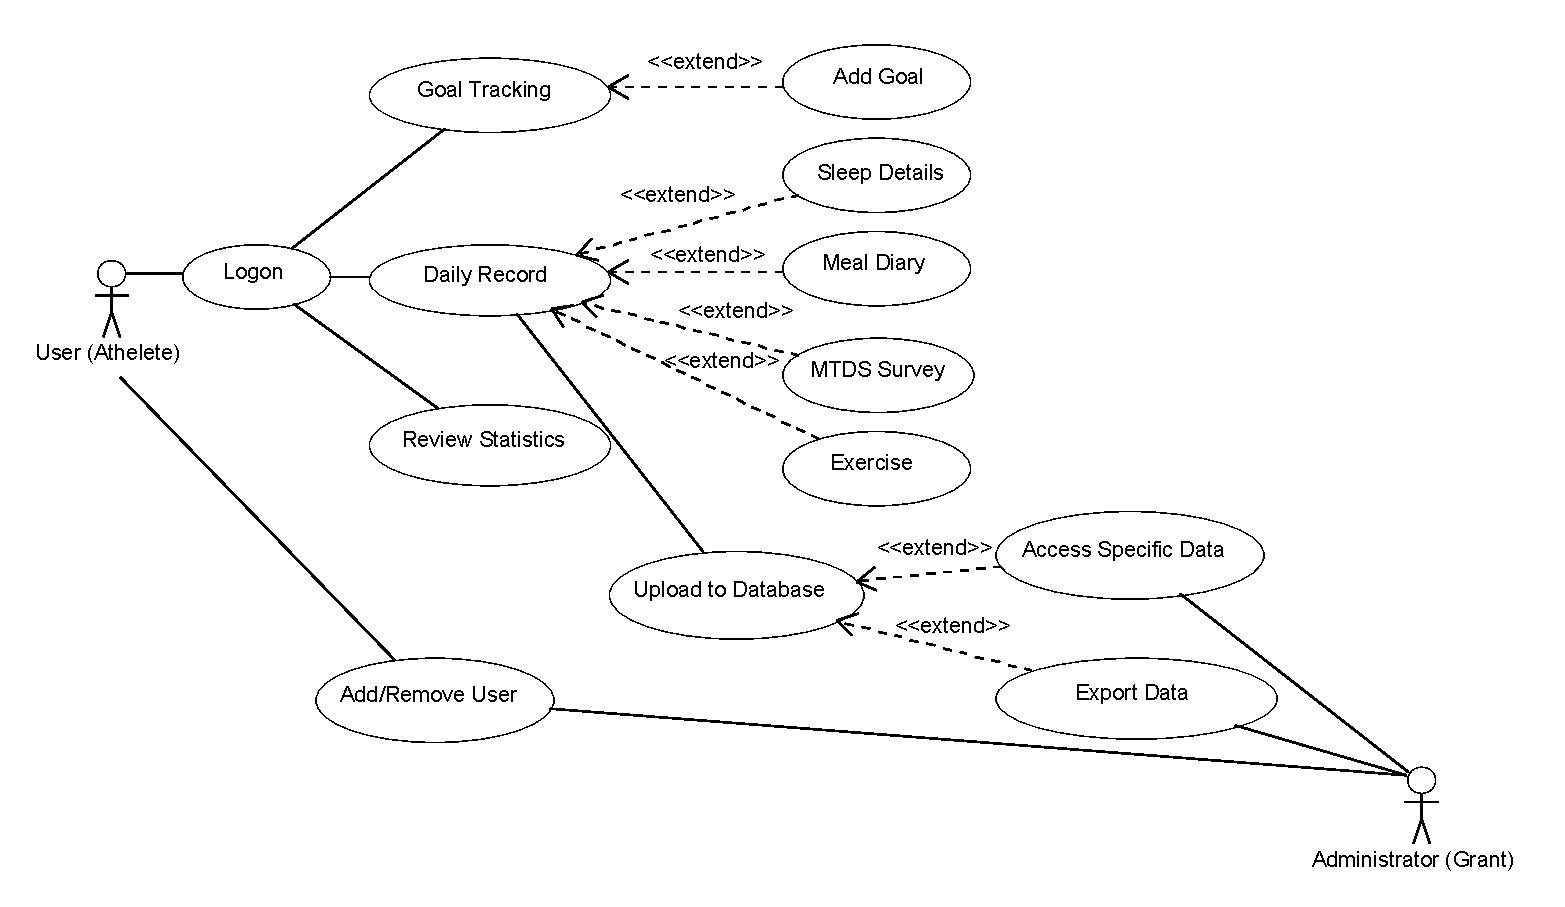
\includegraphics[width=0.9\textwidth]{figures/object-models/use-case.pdf}
	\caption{A use case model of the mobile application}
\end{figure}

 \begin{table}[H]
\begin{tabularx}{\textwidth}{l|X}
& \textbf{Descriptions} \\
\hline
\textbf{Name} & Logon \\
\textbf{Goal} & User is required to logon the system to access any functionality \\
\textbf{Flow of Events} & \begin{tabular}[c]{@{}l@{}}1. After the app is launched, user will land on a splash screen for login.\\ 2. With successful authentication user will be brought to the app interface.\end{tabular} \\
\textbf{Special Requirements} & nil \\
\textbf{Pre-conditions} & Application is launched. \\
\textbf{Post-conditions} & The application functionality will be unlocked.
\end{tabularx}
\end{table}

\begin{table}[H]
\begin{tabularx}{\textwidth}{l|X}
& \textbf{Descriptions} \\ \hline
\textbf{Name} & Goal Tracking \\ 
\textbf{Goal} & User will be able to review/edit goal set previously \\ 
\textbf{Flow of Events} & 1. Click on specific goal to review existing goal \\ 
\textbf{Special Requirements} & nil \\ 
\textbf{Pre-conditions} & Application is launch. And user is in Goal tab. \\ 
\textbf{Post-conditions} & User able to add goal. \\ 
\end{tabularx}
\end{table}

\begin{table}[H]
\begin{tabularx}{\textwidth}{l|l}
& \textbf{Descriptions} \\
\hline
\textbf{Name} & Set goal \\
\textbf{Goal} & User will be able to set a goal \\
\textbf{Flow of Events} & \begin{tabular}[c]{@{}l@{}}1. Click on ``+" to add goal\\ 2. Brought to the add goal screen\\ 3. Fill in detail and submit\\ 4. Goal added\end{tabular} \\
\textbf{Special Requirements} & nil \\
\textbf{Pre-conditions} & Application is launched. User is in Goal tab and has pressed ``+". \\
\textbf{Post-conditions} & New goal added to the App
\end{tabularx}
\end{table}

\begin{table}[H]
\begin{tabularx}{\textwidth}{l|l}
& \textbf{Descriptions} \\
\hline
\textbf{Name} & Meal and sleep diary \\
\textbf{Goal} & User will be able to record meals and sleep details \\
\textbf{Flow of Events} & \begin{tabular}[c]{@{}l@{}}1. Click on ``+" to on every specific tab\\ 2. Brought to the add screen\\ 3. Fill in detail and submit\\ 4. Meal/Sleep details updated\end{tabular} \\
\textbf{Special Requirements} & nil \\
\textbf{Pre-conditions} & Application is launched. And user is in Diary tab and pressed "+". \\
\textbf{Post-conditions} & Meal/Sleep updated to the App
\end{tabularx}
\end{table}

\subsubsection{Object Models}
\paragraph{Data dictionary}
The following describes the proposed layout of the database needed to run this app. 
% Table generated by Excel2LaTeX from sheet 'Sheet1'
\begin{table}[H]
  \centering
  \caption{A list of abbreviations used}
    \begin{tabular}{ll}
    \hline
    Abbreviation & Description \\
    \hline
    NN    & Not null \\
    U     & Unique \\
    255C  & 255 characters \\
    FK(x) & Foreign Key to x \\
    PK    & Primary Key \\
    \hline
    \end{tabular}%
  \label{tab:abbreviations}%
\end{table}%

% Table generated by Excel2LaTeX from sheet 'Sheet1'
\begin{table}[H]
  \centering
  \caption{The \texttt{User} table}
    \begin{tabularx}{\textwidth}{lllXl}
    \hline
    Name  & Restrictions & Data Type & Description & Default value \\
    \hline
    UserID PK & NN, U & Integer & Unique user ID & Next integer \\
    Email & NN, U, 255C & String & User's email address &  \\
    First name & NN, 255C & String & User's first name &  \\
    Last name & NN, 255C & String & User's last name &  \\
    IsAdmin & NN    & Integer & Is the user an administrator? & FALSE \\
    \hline
    \end{tabularx}%
  \label{tab:dd:User}%
\end{table}%


% Table generated by Excel2LaTeX from sheet 'Sheet1'
\begin{table}[H]
  \centering
  \caption{The \texttt{Diary} table}
    \begin{tabularx}{\textwidth}{llp{2.5cm}Xl}
    \hline
    Name  & Restrictions & Data Type & Description & Default value \\
    \hline
    DiaryID PK & NN,U  & Integer & Diary entry unique ID & Next integer \\
    UserID & NN    & Integer, FK(User) & User ID of user who created entry &  \\
    Timestamp & NN    & Date  & Date/time of when the entry was created &  \\
    EntryType & NN    & Integer, FK(DiaryType) & The entry type (e.g. Breakfast, Lunch or Dinner) &  \\
    EntryData & NN, 255C & String & The entry contents (what the user wrote for this entry) &  \\
    \hline
    \end{tabularx}%
  \label{tab:dd:Diary}%
\end{table}%


% Table generated by Excel2LaTeX from sheet 'Sheet1'
\begin{table}[H]
  \centering
  \caption{The \texttt{DiaryType} table.}
    \begin{tabularx}{\textwidth}{lllXl}
    \hline
    Name  & Restrictions & Data Type & Description & Default value \\
    \hline
    DiaryTypeID PK & NN, U & Integer & Diary type unique ID & Next integer \\
    Name  & NN, U, 255C & String & The entry type name (e.g. Breakfast, Lunch or Dinner) &  \\
    Description & 255C  & String & An optional description &  \\
    \hline
    \end{tabularx}%
  \label{tab:dd:DiaryType}%
\end{table}%


% Table generated by Excel2LaTeX from sheet 'Sheet1'
\begin{table}[H]
  \centering
  \caption{The \texttt{DailyStats} table.}
    \begin{tabularx}{\textwidth}{llp{2.5cm}Xl}
    \hline
    Name  & Restrictions & Data Type & Description & Default value \\
    \hline
    StatsID PK & NN, U & Integer & DailyStats unique ID & Next integer \\
    UserID & NN    & Integer, FK(User) & User ID for user that this stats entry belongs to &  \\
    Timestamp & NN    & Date  & Day of stats entry &  \\
    Stats & NN    & String & Serialised statistics (e.g. JSON) &  \\
    \hline
    \end{tabularx}%
  \label{tab:dd:DailyStats}%
\end{table}%


% Table generated by Excel2LaTeX from sheet 'Sheet1'
\begin{table}[H]
  \centering
  \caption{The \texttt{Survey} table.}
    \begin{tabularx}{\textwidth}{lllXl}
    \hline
    Name  & Restrictions & Data Type & Description & Default value \\
    \hline
    SurveyID PK & NN, U & Integer & Survey unique ID & Next integer \\
    Description & NN, 255C & String & Survey description &  \\
    Name  & NN, U, 255C & String & The name of the survey &  \\
    \hline
    \end{tabularx}%
  \label{tab:dd:Survey}%
\end{table}%


% Table generated by Excel2LaTeX from sheet 'Sheet1'
\begin{table}[H]
  \centering
  \caption{The \texttt{SurveyQuestion} table.}
    \begin{tabularx}{\textwidth}{llp{2.5cm}Xl}
    \hline
    Name  & Restrictions & Data Type & Description & Default value \\
    \hline
    QuestionID PK & NN, U & Integer & Question unique ID & Next integer \\
    SurveyID & NN    & Integer, FK(Survey) & Survey ID that this question belongs to &  \\
    QuestionText & NN    & String & The question text &  \\
    QuestionType & NN    & String & The question type (e.g. radio, multi-choice, number) &  \\
    Choices & 255C  & String & Comma separated list of choices (if type is suitable) &  \\
    Required & NN    & Boolean & Is this question required? & TRUE \\
    \hline
    \end{tabularx}%
  \label{tab:dd:SurveyQuestion}%
\end{table}%


% Table generated by Excel2LaTeX from sheet 'Sheet1'
\begin{table}[H]
  \centering
  \caption{The \texttt{SurveyResponse} table.}
    \begin{tabularx}{\textwidth}{llp{2.5cm}Xl}
    \hline
    Name  & Restrictions & Data Type & Description & Default value \\
    \hline
    ResponseID PK & NN, U & Integer & Survey response unique ID & Next integer \\
    SurveyID & NN    & Integer, FK(Survey) & ID of survey that this response corresponds to &  \\
    UserID & NN    & Integer, FK(User) & ID of user who completed this response &  \\
    Timestamp & NN    & Date  & Date/time of when this response was completed &  \\
    \hline
    \end{tabularx}%
  \label{tab:dd:SurveyResponse}%
\end{table}%


% Table generated by Excel2LaTeX from sheet 'Sheet1'
\begin{table}[H]
  \centering
  \caption{The \texttt{QuestionResponse} table.}
    \begin{tabularx}{\textwidth}{llp{3.3cm}Xl}
    \hline
    Name  & Restrictions & Data Type & Description & Default value \\
    \hline
    QResponseID PK & NN, U & Integer & QuestionResponse unique ID & Next integer \\
    ResponseID & NN    & Integer, FK(SurveyResponse) & ID of response that this is part of &  \\
    QuestionID & NN    & Integer, FK(SurveyQuestion) & ID of question that this is answering &  \\
    Answer & NN, 255C & String & The answer to the question &  \\
    \hline
    \end{tabularx}%
  \label{tab:dd:QuestionResponse}%
\end{table}%

Note that the \texttt{User} table is only given as an example of what is required from it. Most frameworks already provide an implementation for users (and the associated table). 

\paragraph{Class diagrams}
The database must allow for user management, storage of surveys (MTDS/Sleep/Training volume) and their responses, as well as storage of diary entries. For ease of access, an additional table storing aggregated statistics based on the survey responses is also kept.

\begin{figure}[H]
	\centering
	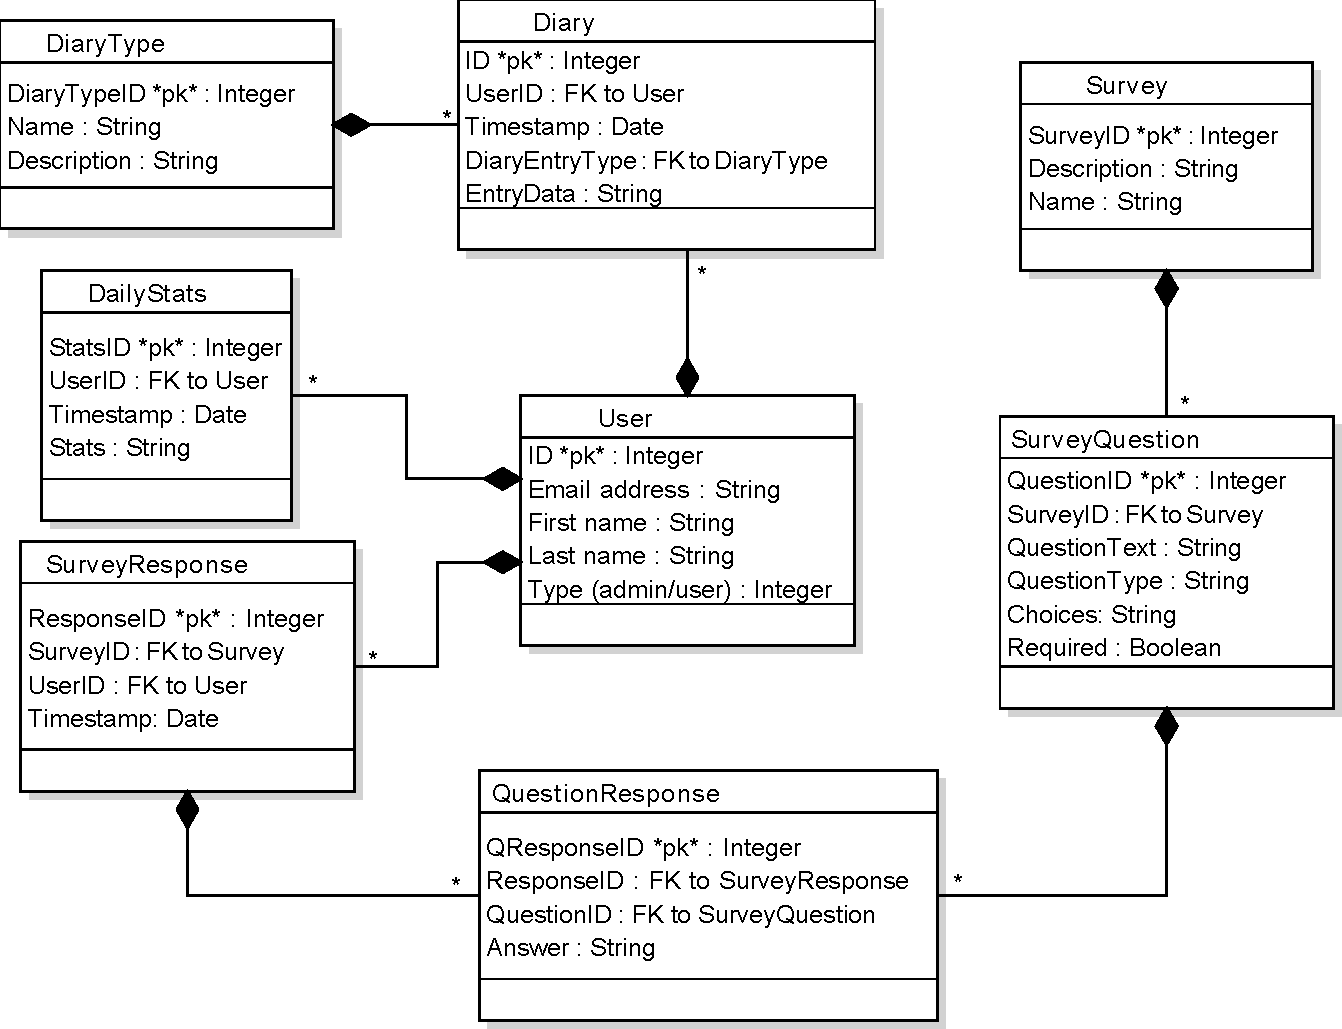
\includegraphics[width=0.8\textwidth]{figures/object-models/db-schema.pdf}
	\caption{The proposed database table layout}
\end{figure}

The mobile application uses an MVC framework. What follows is a list of views and the required functions from the controllers (in UML) in the app.

\begin{figure}[H]
	\centering
	\begin{tabular}{ccc}
	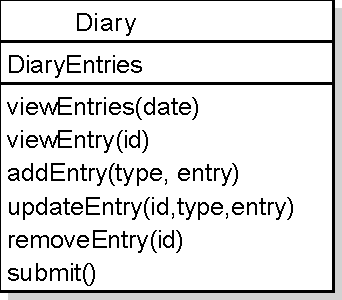
\includegraphics[width=0.25\textwidth]{figures/object-models/AppDiary.pdf} A & 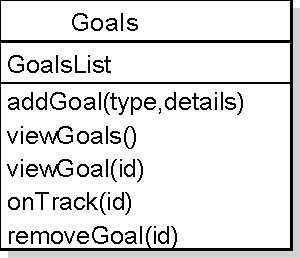
\includegraphics[width=0.25\textwidth]{figures/object-models/AppGoals.pdf} B & 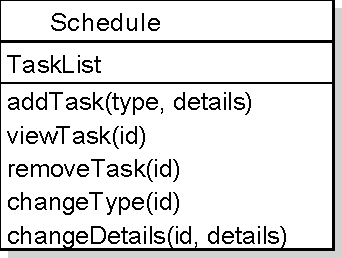
\includegraphics[width=0.25\textwidth]{figures/object-models/AppSchedule.pdf} C \\
	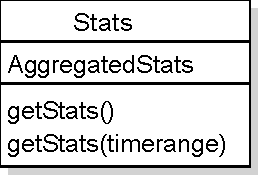
\includegraphics[width=0.25\textwidth]{figures/object-models/AppStats.pdf} D & 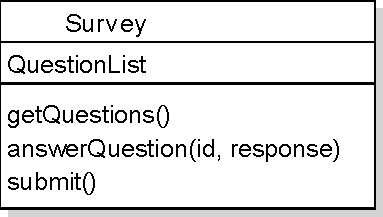
\includegraphics[width=0.25\textwidth]{figures/object-models/AppSurvey.pdf} E
	\end{tabular}
	\caption{A set of views required by the app}
\end{figure}

\newpage
\subsubsection{Dynamic Models}
The following models provide examples of the sequence of steps behind a user interacting with the app, under various scenarios.
\begin{figure}[H]
	\centering
	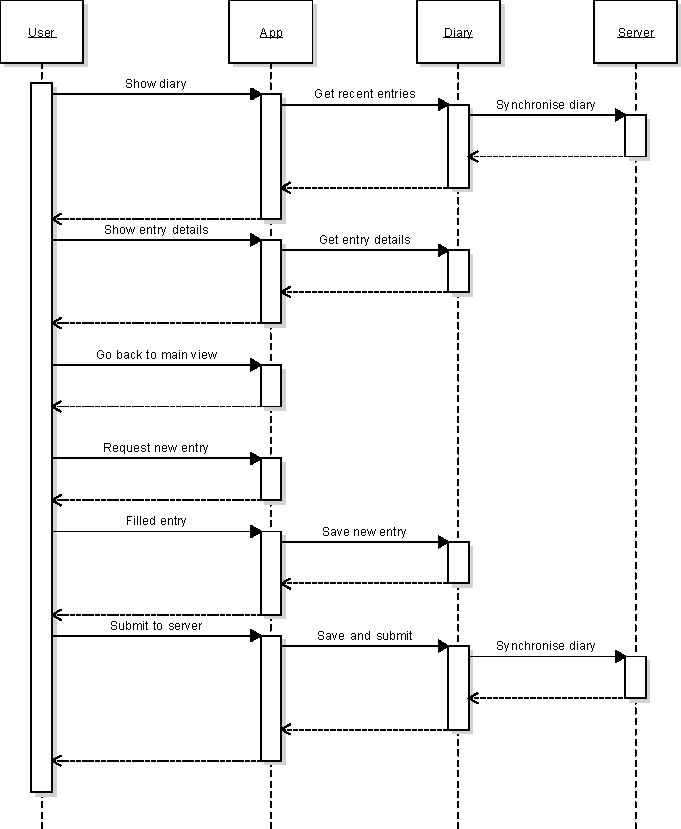
\includegraphics[width=0.8\textwidth]{figures/sequence-diagrams/AppDiarySeq.pdf}
	\caption{A sequence diagram of a user viewing the diary and one entry, before filling in a new entry and submitting it to the server.}
\end{figure}

\begin{figure}[H]
	\centering
	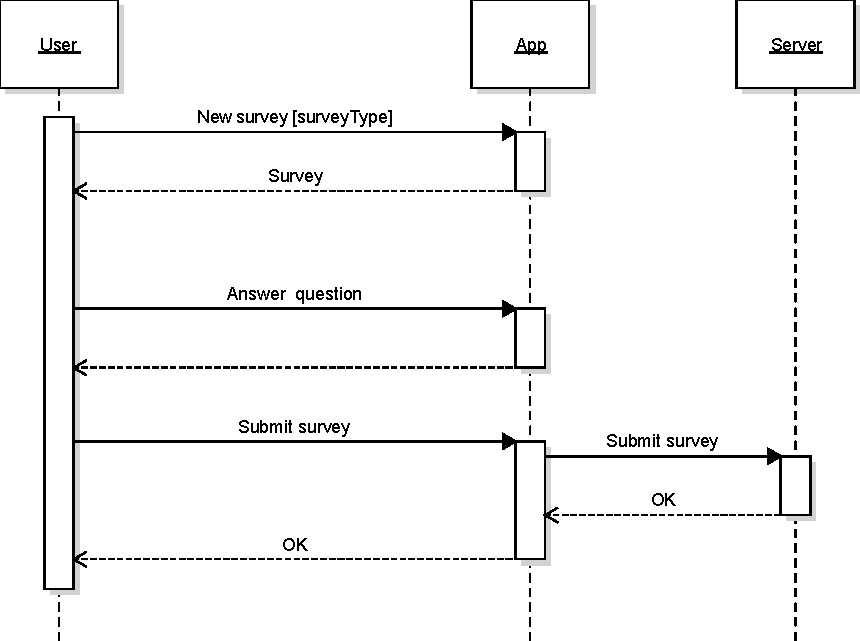
\includegraphics[width=0.7\textwidth]{figures/sequence-diagrams/AppSurveySeq.pdf}
	\caption{A sequence diagram of a user completing a new sleep quality survey and submitting it to the server.}
\end{figure}

\begin{figure}[H]
	\centering
	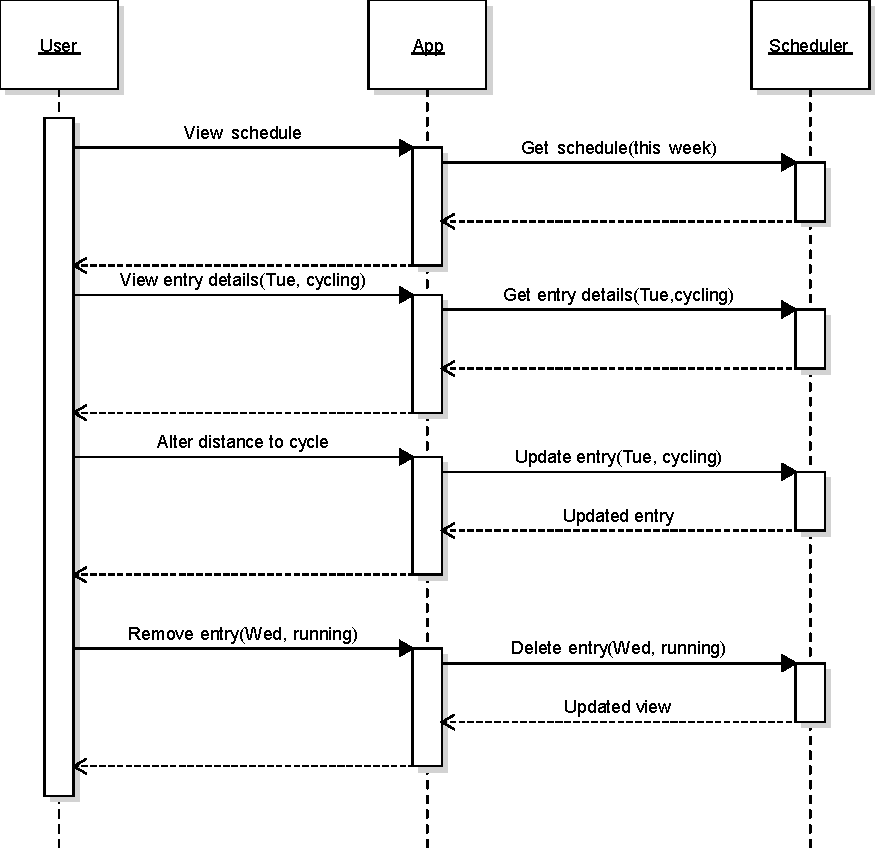
\includegraphics[width=0.66\textwidth]{figures/sequence-diagrams/AppScheduleSeq.pdf}
	\caption{A sequence diagram of interaction with the timetable. In this example, the user views this week's overview, then views the details for one entry (cycling on Tuesday). After viewing the entry, the user alters the distance that he/she plans to cycle. The user then removes another entry (running on Wednesday).}
\end{figure}

\begin{figure}[H]
	\centering
	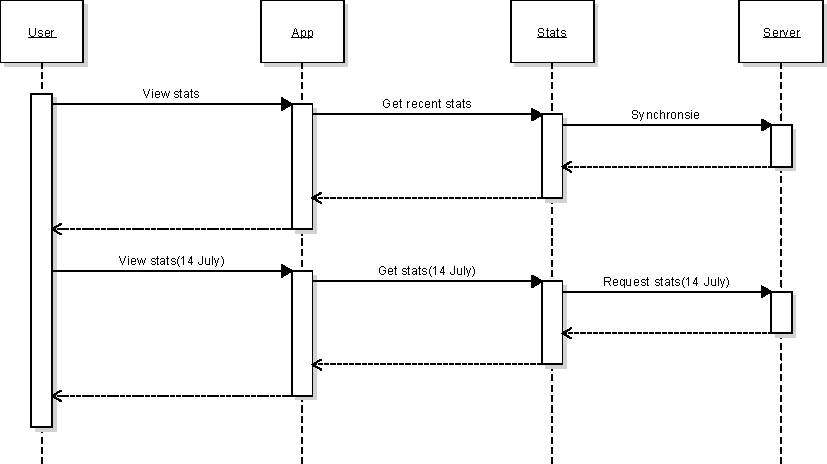
\includegraphics[width=0.8\textwidth]{figures/sequence-diagrams/AppStatsSeq.pdf}
	\caption{A sequence diagram of a user viewing recent stats and stats for a particular time frame.}
\end{figure}

\begin{figure}[H]
	\centering
	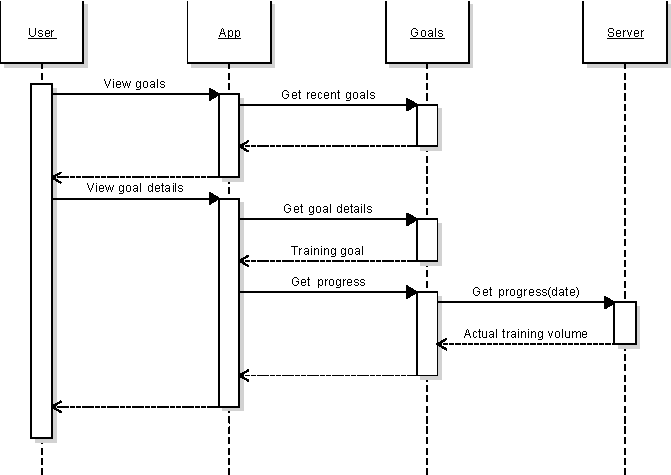
\includegraphics[width=0.8\textwidth]{figures/sequence-diagrams/AppGoalsSeq.pdf}
	\caption{A sequence diagram of a user viewing their training goals.}
\end{figure}


\subsubsection{User Interface --- Navigational Paths and Screen Mock-ups}
\begin{figure}[H]
	\centering
	
	\begin{tabular}{cc}
		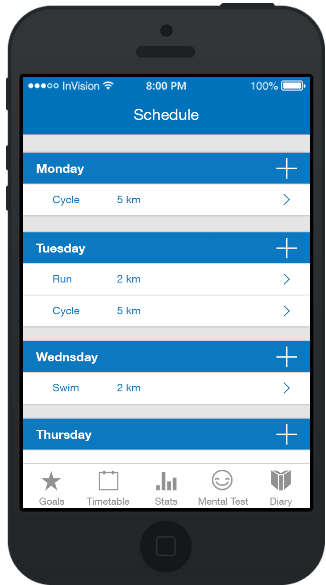
\includegraphics[width=0.36\textwidth]{figures/mockups/schedule-1.png} A &
		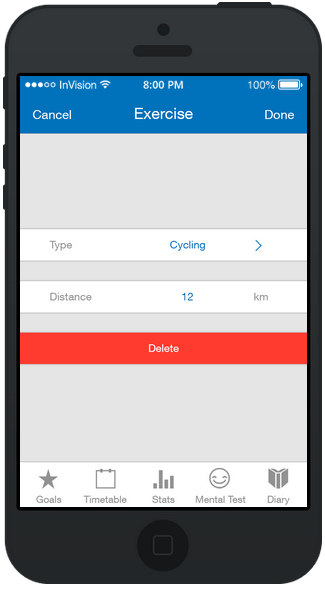
\includegraphics[width=0.36\textwidth]{figures/mockups/schedule-2.png} B \\
		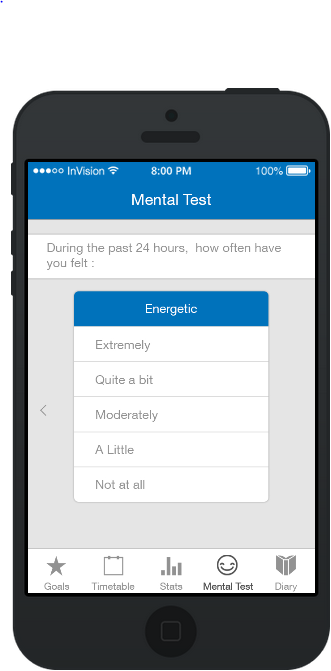
\includegraphics[width=0.36\textwidth]{figures/mockups/mtds-1.png} C &
		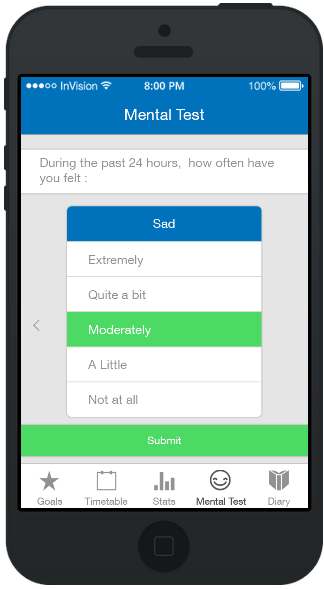
\includegraphics[width=0.36\textwidth]{figures/mockups/mtds-2.png} D 
	\end{tabular}
	\caption{Mock-ups of the app}
	\label{fig:mockups}
\end{figure}

\begin{figure}[H]
	\centering
	
	\begin{tabular}{cc}
		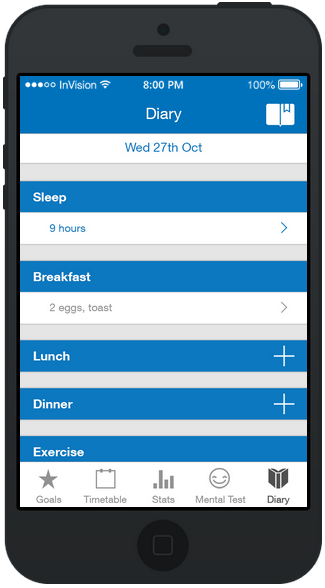
\includegraphics[width=0.38\textwidth]{figures/mockups/diary-1.png} E &
		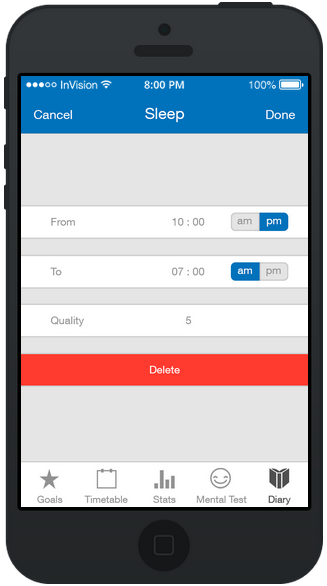
\includegraphics[width=0.38\textwidth]{figures/mockups/diary-2.png} F \\
		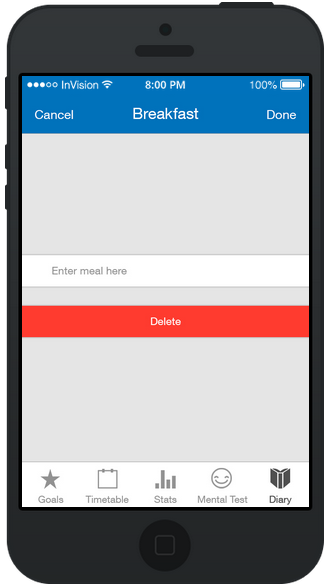
\includegraphics[width=0.38\textwidth]{figures/mockups/diary-3.png} G &
		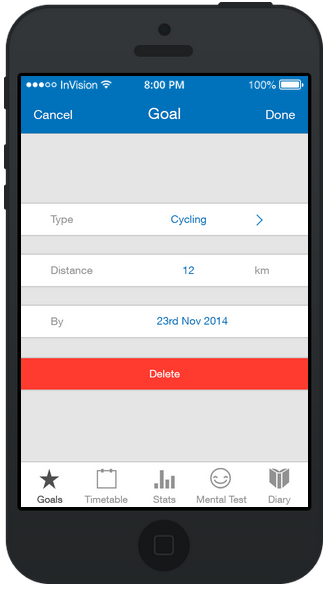
\includegraphics[width=0.38\textwidth]{figures/mockups/goal-1.png} H
	\end{tabular}

	\caption{Mock-ups of the app (continued)}
	\label{fig:mockups-2}
\end{figure}

Mockups A and B shows the design of the schedule feature and entry of a new item. Mockups C and D provide a sample design for filling out the MTDS survey. The diary feature is shown in Mockups E-G, with filling out the sleep survey in mockup F. The goal feature is shown in Mockup H.

\pagebreak
\section{Glossary}
\begin{itemize}
	\item \textbf{Android} --- A mobile operating system developed by Google. Used on most non-Apple branded phones and tablets.
	\item \textbf{app} --- `Mobile application'; software than runs on a smart phone.
	\item \textbf{CSS} --- Cascading Style Sheets -- A language used to format how a document appears; typically used with HTML.
	\item \textbf{CSV} --- Comma Separated Values -- A common and simple format to export data to; rows are entered one per line, and columns are separated by a delimiter (i.e. a comma).
	\item \textbf{HTML} --- HyperText Markup Language -- A markup language used to create web pages.
	\item \textbf{Ionic} --- A framework to design cross-platform mobile applications using HTML, CSS and JavaScript.
	\item \textbf{iOS} --- A mobile operating system developed by Apple. Used on all Apple mobile products (iPhone/iPad)
	\item \textbf{JavaScript} --- A scripting language often used to control web pages, making them interactive.
	\item \textbf{MTDS}
	\item \textbf{MVC} --- Model-View-Controller. A framework that presents a `view' of a `model' to the user. The user interacts with the `view', which is made interactive/controlled by the `controller', which then updates the `model'.
	\item \textbf{SQL} --- Structured Query Language -- A programming language used in the control of a relational database management system.
	\item \textbf{UML} --- Unified Modeling Language -- A general-purpose method of visualising the design of a system.
	\item \textbf{UWA} --- The University of Western Australia.
\end{itemize}

%Referencing
% Commented out - no referencing so far
%---------------------------------------------------------
%\renewcommand{\refname}{References}
%\bibliographystyle{apalike}
%\bibliography{references/refs}

%\addbibresource{references/refs.bib}
%\printbibliography
%\addcontentsline{toc}{part}{References}
%---------------------------------------------------------

\end{document}